\section{Experimentación con el filtro adaptativo}

En la presente sección se describe el proceso de experimentación llevado a cabo para evaluar el rendimiento del filtro adaptativo.

Para la evaluación se utilizó la base de datos construida a partir del proceso descrito en la sección \ref{sec:audio_db}.

La base de datos fue dividida en dos conjuntos disjuntos:

\begin{itemize}
	\item Conjunto de entrenamiento: El filtro basado en redes neuronales depende de un conjunto de entrenamiento que se encarga de optimizar los parámetros de la red de tal manera que el error sea el menor posible. El filtro adaptativo no requiere de un conjunto de entrenamiento ya que sus parámetros son optimizados en tiempo real.
	\item Conjunto de prueba: Para evaluar cada filtro de manera objetiva, se utiliza el conjunto de pruebas.
\end{itemize}

Una división comúnmente utilizada es la de asignar el 70\% de las muestras en el conjunto de entrenamiento y el 30\% restante, utilizarlo para el conjunto de prueba. Dicha práctica fue la utilizada en el presente trabajo.

El proceso de pruebas consistió en ingresar al filtro adaptativo señales ruidosas, obtener la respuesta del filtro y compararla con la señal original sin ruido, por medio de las métricas STOI y PESQ.

\subsection{Parámetros del filtro}

De las ecuaciones vistas en la sección \ref{sec:filtro_adaptativo_procesamiento_de_señales} se observa que antes de poder utilizar el filtro, se necesitan definir algunos parámetros:

\begin{itemize}
	\item Cantidad de coeficientes $M$.
	\item Factor de olvido $\lambda$.
	\item Factor de regularización $\epsilon$.
\end{itemize}


A continuación veremos cómo se configuraron cada uno de ellos.

\subsubsection{Cantidad de coeficientes $M$}

El parámetro M define el largo del filtro y por ende la cantidad de coeficientes. A mayor cantidad de coeficientes mayor será la capacidad del filtro para adaptarse a los retardos entre las señales captadas por los micrófonos y también será mayor la capacidad de cancelación. Sin embargo, a medida que aumentamos la cantidad de coeficientes, también aumenta el tiempo de procesamiento. Para el presente trabajo se utilizaron 16 coeficientes, es decir $M=16$.

\subsubsection{Factor de olvido $\lambda$}

El factor de olvido $\lambda$ se debe escoger en el rango $0 \ll \lambda \le 1$. En el caso extremo de $\lambda=1$, la estimación de la matriz de autocorrelación adopta el valor

\begin{equation*}
	\hat{R}_{uu} = \frac{1}{i+1} \sum_{j=0}^{i} u_j^* u_j
\end{equation*}

\noindent es decir, se promedian todas las estimaciones anteriores de $R_{uu}$. Al elegir un valor menor a uno, se dice que se le introduce memoria a la estimación ya que se le estará dando mayor importancia a las estimaciones recientes que a las pasadas. 

El parámetro $\lambda$ define la capacidad de adaptación del algoritmo. Mientras más cerca de uno esté, más lento responderá el filtro ante cambios en las características de la señal de entrada $u$. Para el presente trabajo se encontró que una buena relación de compromiso se encuentra en el valor $\lambda=0.998$.

\subsubsection{Factor de regularización $\epsilon$}

En la sección \ref{sec:adaptive_filter_rls} vimos que, desde el punto de vista de los filtros adaptativos, el filtro RLS surge de la recursión de Newton dada por:

\begin{equation}
	w_i = w_{i-1} + \mu (\epsilon I + R_{uu} )^{-1} \left( R_{du} - R_{uu} w_{i-1} \right)
\end{equation}

El término $\epsilon I$ permite regularizar la inversión de la matriz que estima $R_{uu}$, es decir regularizar la inversa de:

\begin{equation*}
	\hat{R}_{uu} = \frac{1}{i+1} \sum_{j=0}^{i} u_j^* u_j
\end{equation*}

Desarrollando la recursión y eligiendo $\epsilon(i) = \frac{\lambda^{i+1} \epsilon }{i+1}$ se obtiene que el parámetro $\epsilon$ sólo está involucrado en la condición inicial del algoritmo. Un valor usualmente utilizado y que en el presente trabajo permitió la adecuada regularización, es el de $\epsilon=0.01$


\subsection{Resultados}

\subsubsection{Medida PESQ}

Dado el conjunto de audios de prueba con un largo igual a $P$, las señales de habla ruidosas $d_p(n)$, y las señales de habla filtradas $\hat{s}_p(n)$, se definieron las siguientes seis medidas:

\begin{itemize}
	\item $\textbf{Min PESQ}$: Medida PESQ entre la señal de habla ruidosa y la señal de habla sin ruido. Establece una cota inferior en la medida PESQ que debería tener la señal de habla filtrada.
	\item $\textbf{Min PESQ Valor medio}$: Valor medio de la medida $\textbf{Min PESQ}$.
	\item $\textbf{PESQ}$: Medida PESQ entre la señal de habla filtrada y la señal de habla sin ruido.
	\item $\textbf{PESQ Valor medio}$: Valor medio de la medida $\textbf{PESQ}$.
	\item $\Delta \textbf{PESQ}$: Mejora en la medida \textbf{PESQ} por efecto del filtro.
	\item $\Delta \textbf{PESQ Valor medio}$: Valor medio de la medida $\Delta \textbf{PESQ}$.
\end{itemize}

Formalmente:

\begin{itemize}
	\item $\textbf{Min PESQ} = PESQ\{ d_p(n) \}$
	\item $\textbf{Min PESQ Valor medio} = \frac{1}{P-1} \sum_{p=0}^{P-1} PESQ\{ d_p(n) \}$
	\item $\textbf{PESQ} = PESQ\{ \hat{s}_p(n) \}$
	\item $\textbf{PESQ Valor medio} = \frac{1}{P-1} \sum_{p=0}^{P-1} PESQ\{ \hat{s}_p(n) \}$
	\item $\Delta \textbf{PESQ} = \left( PESQ\{ \hat{s}_p(n) \} - PESQ\{ d_p(n) \} \right)$
	\item $\Delta \textbf{PESQ Valor medio} = \frac{1}{p-1} \sum_{p=0}^{P-1} \left( PESQ\{ \hat{s}_p(n) \} - PESQ\{ d_p(n) \} \right)$
\end{itemize}

Uno de los objetivos del filtro de ruido es mejorar, o al menos mantener, la calidad de la señal de habla, es por eso que la medida PESQ calculada para la señal ruidosa $d(n)$ nos da una cota inferior, es decir se espera que:

\begin{equation*}
	PESQ\{ \hat{s}_p(n) \} \geq PESQ\{ d_p(n) \}
\end{equation*}

El valor $\Delta \textbf{PESQ Valor medio}$ nos dirá en promedio cuánto logrará mejorar la PESQ, el filtro en evaluación.

Como vimos en la sección \ref{sec:metrics}, las señales de habla ruidosa fueron construidas utilizando distintos valores de SNR. Una forma de evaluar el filtro es analizar qué tanto cambia la PESQ para cada valor de SNR utilizado.

En la figura \ref{fig:ch6_pesq_resume} podemos ver la medida $\Delta \textbf{PESQ Valor medio}$ para el total de señales de habla, para cada valor de SNR. En la gráfica se observa que una vez superado los $\SI{15}{dB}$, el filtro empeoró la calidad de las señales de audio.

\begin{figure}
	\centering
	\centerline{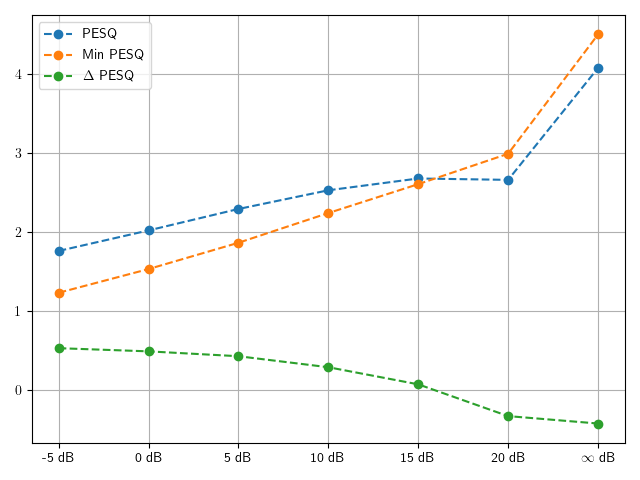
\includegraphics[scale=0.75]{images/ch6/af/objective_metrics/metric_PESQ.png}}
	\caption{PESQ en función de la SNR.}
	\label{fig:ch6_pesq_resume}
\end{figure}

A medida que la SNR fue aumentando, le resultó cada vez más difícil al filtro poder mejorar el valor de base de la medida $PESQ$. Incluso en los casos de $SNR = \SI{20}{dB}$ y $SNR = \inf \; dB$, el filtro la empeoró. En la siguiente sección se analiza este comportamiento mas en detalle.

En la tabla \ref{table:pesq_resume} podemos ver los mismos resultados que en la figura \ref{fig:ch6_pesq_resume} pero en valores porcentuales.

\begin{table}[ht]
	\centering
	\begin{tabular}{ |c|c|c|c|c|c|c|c| } 
		\hline
		SNR [dB] & $-5$ & $0$ & $5$ & $10$ & $15$ & $20$ & $\inf$ \\ 
		\hline
		$\Delta \textbf{PESQ Valor medio}$ & 43\%  & 32\% & 23\% & 13\% & 3\% & -12\% & -10\% \\ 
		\hline
	\end{tabular}
	\caption{Medida $\Delta \textbf{PESQ Valor medio}$ para cada valor de SNR.}
	\label{table:pesq_resume}
\end{table}

Otra forma de evaluar el filtro es analizar cómo varían las medidas en función del tipo de ruido. En la figura \ref{fig:ch6_pesq_resume_by_noise} podemos ver la medida PESQ en función del tipo de ruido.

\begin{figure}
	\centering
	\centerline{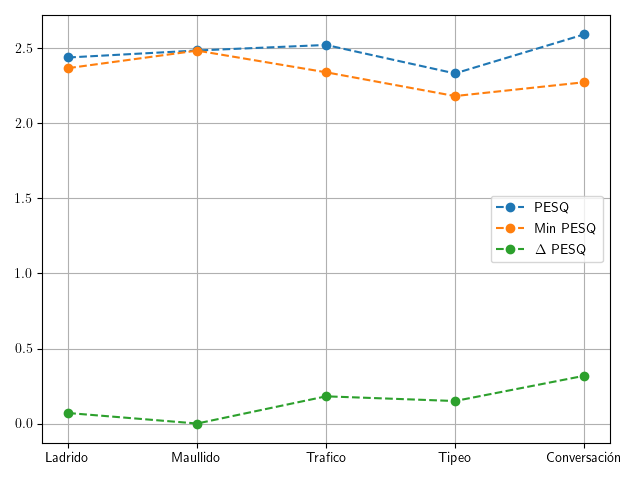
\includegraphics[scale=0.75]{images/ch6/af_metric_PESQ_noises.png}}
	\caption{PESQ en función del tipo de ruido.}
	\label{fig:ch6_pesq_resume_by_noise}
\end{figure} 

Si bien los resultados obtenidos son relativamente constantes para cada uno de los tipos de ruido, se observa un mejor desempeño en el ruido del tipo \emph{Tráfico}, en \emph{Tipeo} y en \emph{Conversación}. Los ruidos del tipo \emph{Ladrido} y \emph{Maullido} tienen la característica de ser de corta duración, lo que representa un inconveniente para el filtro adaptativo que necesita cierto tiempo para adaptarse a las nuevas condiciones de ruido y filtrarlo.

\subsubsection{Medida STOI}

Al igual que para la PESQ, se analizaron las siguientes seis medidas relacionadas con la STOI:

\begin{itemize}
	\item $\textbf{Min STOI} = STOI\{ d_p(n) \}$
	\item $\textbf{Min STOI Valor medio} = \frac{1}{P-1} \sum_{p=0}^{P-1} STOI\{ d_p(n) \}$
	\item $\textbf{STOI} = STOI\{ \hat{s}_p(n) \}$
	\item $\textbf{STOI Valor medio} = \frac{1}{P-1} \sum_{p=0}^{P-1} STOI\{ \hat{s}_p(n) \}$
	\item $\Delta \textbf{STOI} = \left( STOI\{ \hat{s}_p(n) \} - STOI\{ d_p(n) \} \right)$
	\item $\Delta \textbf{STOI Valor medio} = \frac{1}{P-1} \sum_{p=0}^{P-1} \left( STOI\{ \hat{s}_p(n) \} - STOI\{ d_p(n) \} \right)$
\end{itemize}

En la figura \ref{fig:ch6_stoi_resume} podemos ver la medida $\Delta \textbf{STOI Valor medio}$ como función de la SNR. Al igual que para la PESQ, a partir de los $\SI{15}{dB}$ el filtro en lugar de mejorar la inteligibilidad, la empeora.

\begin{figure}
	\centering
	\centerline{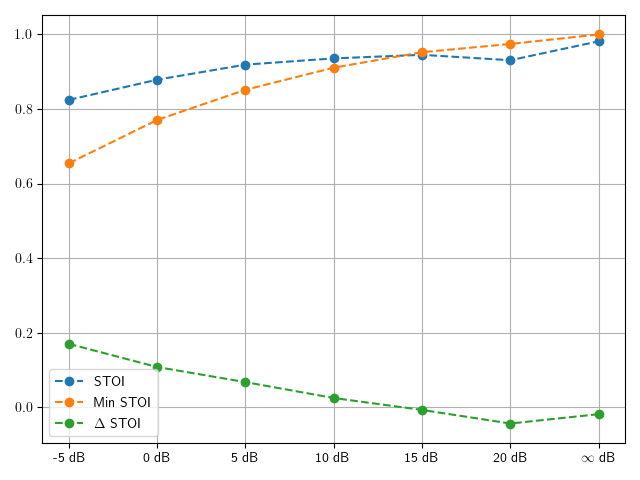
\includegraphics[scale=0.75]{images/ch6/af/objective_metrics/metric_STOI.png}}
	\caption{STOI en función de la SNR.}
	\label{fig:ch6_stoi_resume}
\end{figure}

En la tabla \ref{table:stoi_resume} podemos ver los mismos resultados que en la figura \ref{fig:ch6_stoi_resume} pero en valores porcentuales.

\begin{table}[ht]
	\centering
	\begin{tabular}{ |c|c|c|c|c|c|c|c| } 
		\hline
		SNR [dB] & $-5$ & $0$ & $5$ & $10$ & $15$ & $20$ & $\inf$ \\ 
		\hline
		$\Delta \textbf{STOI Valor medio}$ & 26\%  & 14\%  & 8\% & 2\% & -1\% & -4\% & -2\% \\
		\hline
	\end{tabular}
	\caption{Medida $\Delta \textbf{STOI Valor medio}$ para cada valor de SNR.}
	\label{table:stoi_resume}
\end{table}

También se analizó la medida STOI como función del tipo de ruido. En la figura \ref{fig:ch6_stoi_resume_by_noise} podemos ver dicha gráfica. Se observa la misma tendencia que para la medida PESQ, es decir, el desempeño en los ruidos \emph{Tráfico}, \emph{Tipeo} y \emph{Conversación} fue levemente mejor que en \emph{Ladrido} y \emph{Maullido}.

\begin{figure}
	\centering
	\centerline{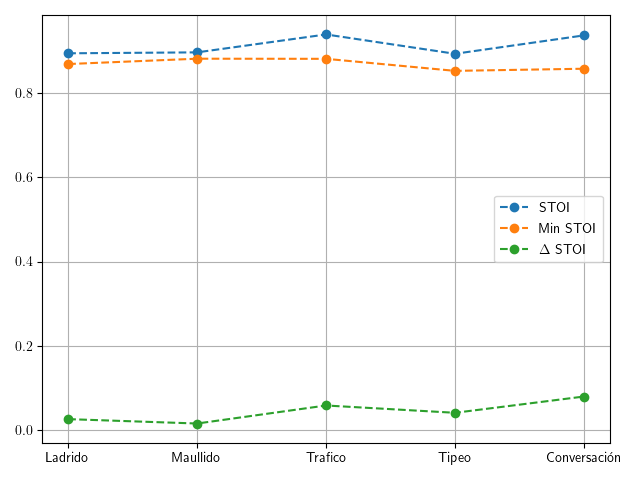
\includegraphics[scale=0.75]{images/ch6/af_metric_STOI_noises.png}}
	\caption{STOI en función del tipo de ruido.}
	\label{fig:ch6_stoi_resume_by_noise}
\end{figure} 

\subsubsection{Error cuadrático medio y nivel de ruido}

Dada la señal de habla sin ruido $s_p(n)$, la señal filtrada $\hat{s}_p(n)$ y $P$ la cantidad de señales de audio en la base de datos de pruebas, se computa el error cuadrático medio como:

\begin{equation*}
	\text{ECM}(n) = \frac{1}{P-1} \sum_{p=0}^{P} (\hat{s}_p(n) - s_p(n))^2
\end{equation*}

También definimos el nivel de ruido medio al cuadrado como:

\begin{equation*}
	\text{Nivel de ruido}(n) = \frac{1}{P-1} \sum_{p=0}^{P} (n_p(n))^2
\end{equation*}

En la figura \ref{fig:ch6_mse_and_noise_level} podemos ver seis gráficas que contiene el error cuadrático medio y el nivel de ruido para cada SNR.

\begin{figure}
	\centering
	\centerline{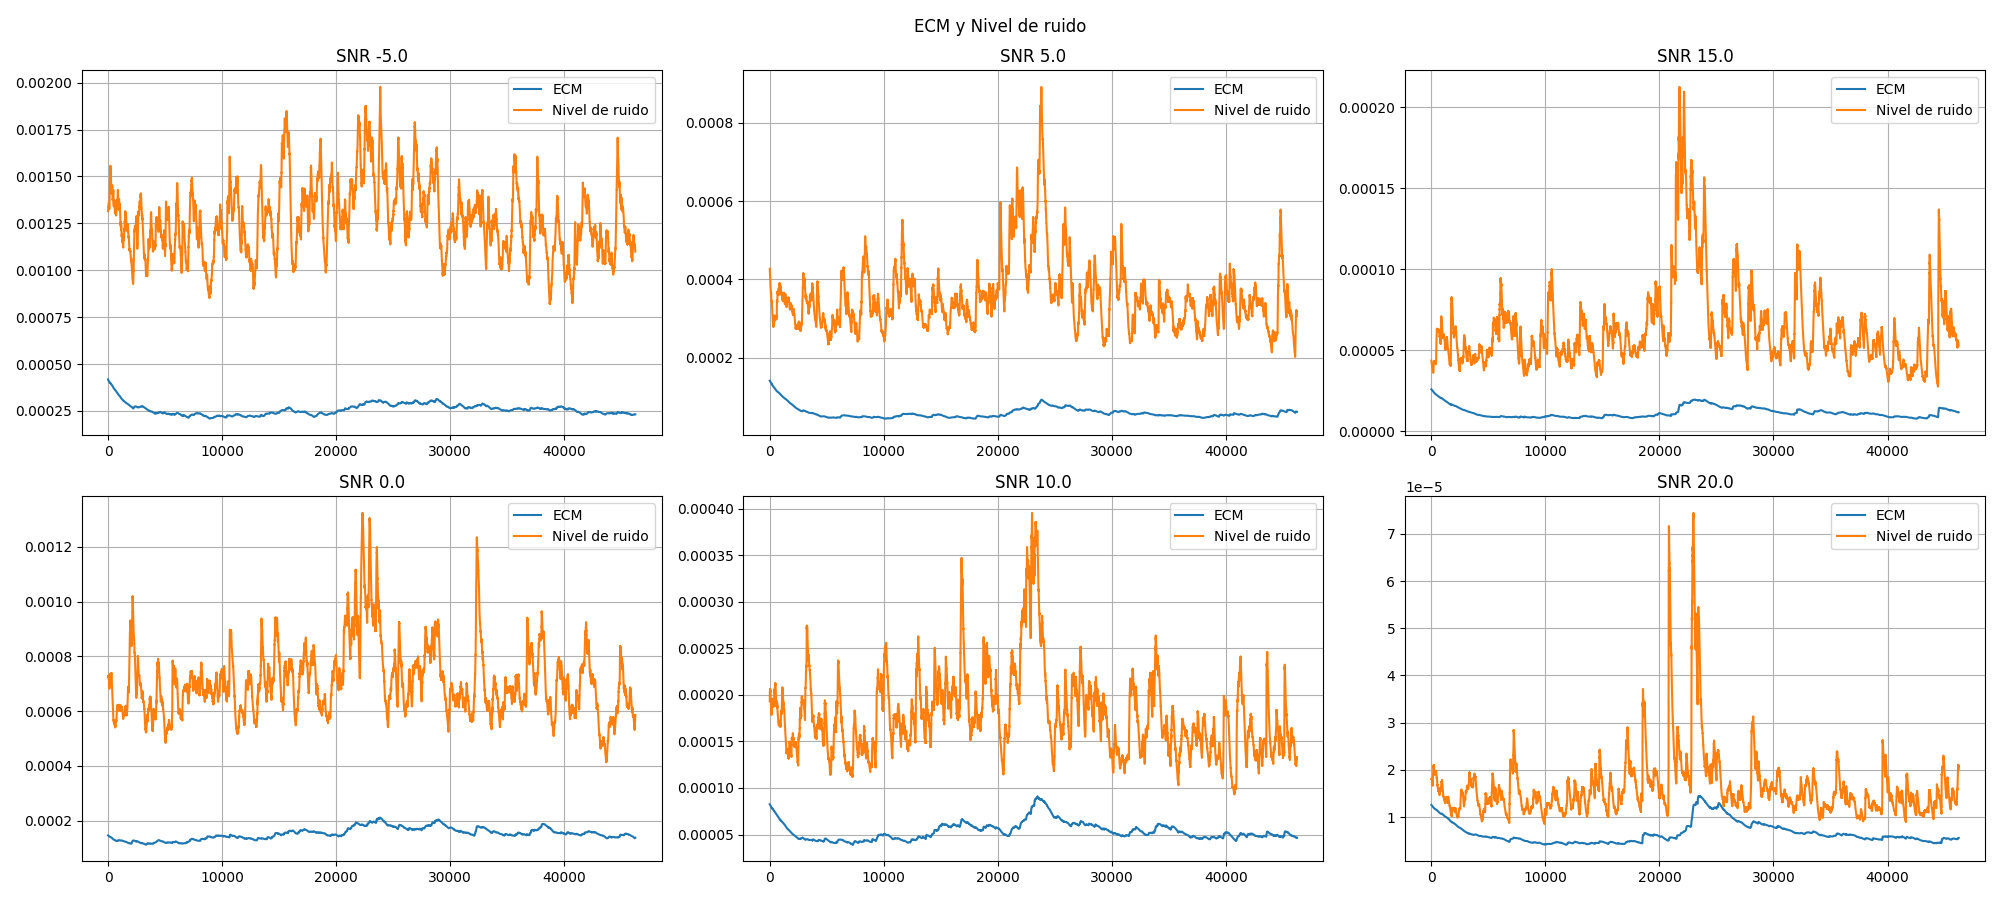
\includegraphics[scale=0.35]{images/ch6/af/mse_and_noise_level.png}}
	\caption{ECM y Nivel de ruido.}
	\label{fig:ch6_mse_and_noise_level}
\end{figure}

En las figuras \ref{fig:ch6_pesq_resume} y \ref{fig:ch6_stoi_resume} vimos que a medida que la SNR aumentó, al filtro le resultó cada vez más difícil lograr una mejora en las medidas PESQ y STOI. Una explicación a este comportamiento lo podemos ver en la figura \ref{fig:ch6_mse_and_noise_level}, donde observamos que a medida que la SNR aumenta, el error cuadrático medio se vuelve comparable con el nivel ruido. Esto lleva a que las medidas $\Delta \textbf{PESQ Valor medio}$ y $\Delta \textbf{STOI Valor medio}$ se acerquen a cero o incluso se vuelvan negativas. En estos casos, la señal de habla filtrada tiene un nivel de ruido similar a la señal de habla ruidosa original, pero esta vez inducido por el error en estado estacionario del filtro adaptativo \cite{fundamentals_of_adaptive_filtering}.

\subsubsection{Variación de los coeficientes en función del tiempo}

Es interesante ver cómo se comportan los coeficientes del filtro para algunos ejemplos concretos. En la figura \ref{fig:ch6_variacion_temporal_de_coeficientes}  podemos ver la variación de los coeficientes del filtro en función del tiempo para 4 audios distintos. 

\begin{figure}
	\centering
	\centerline{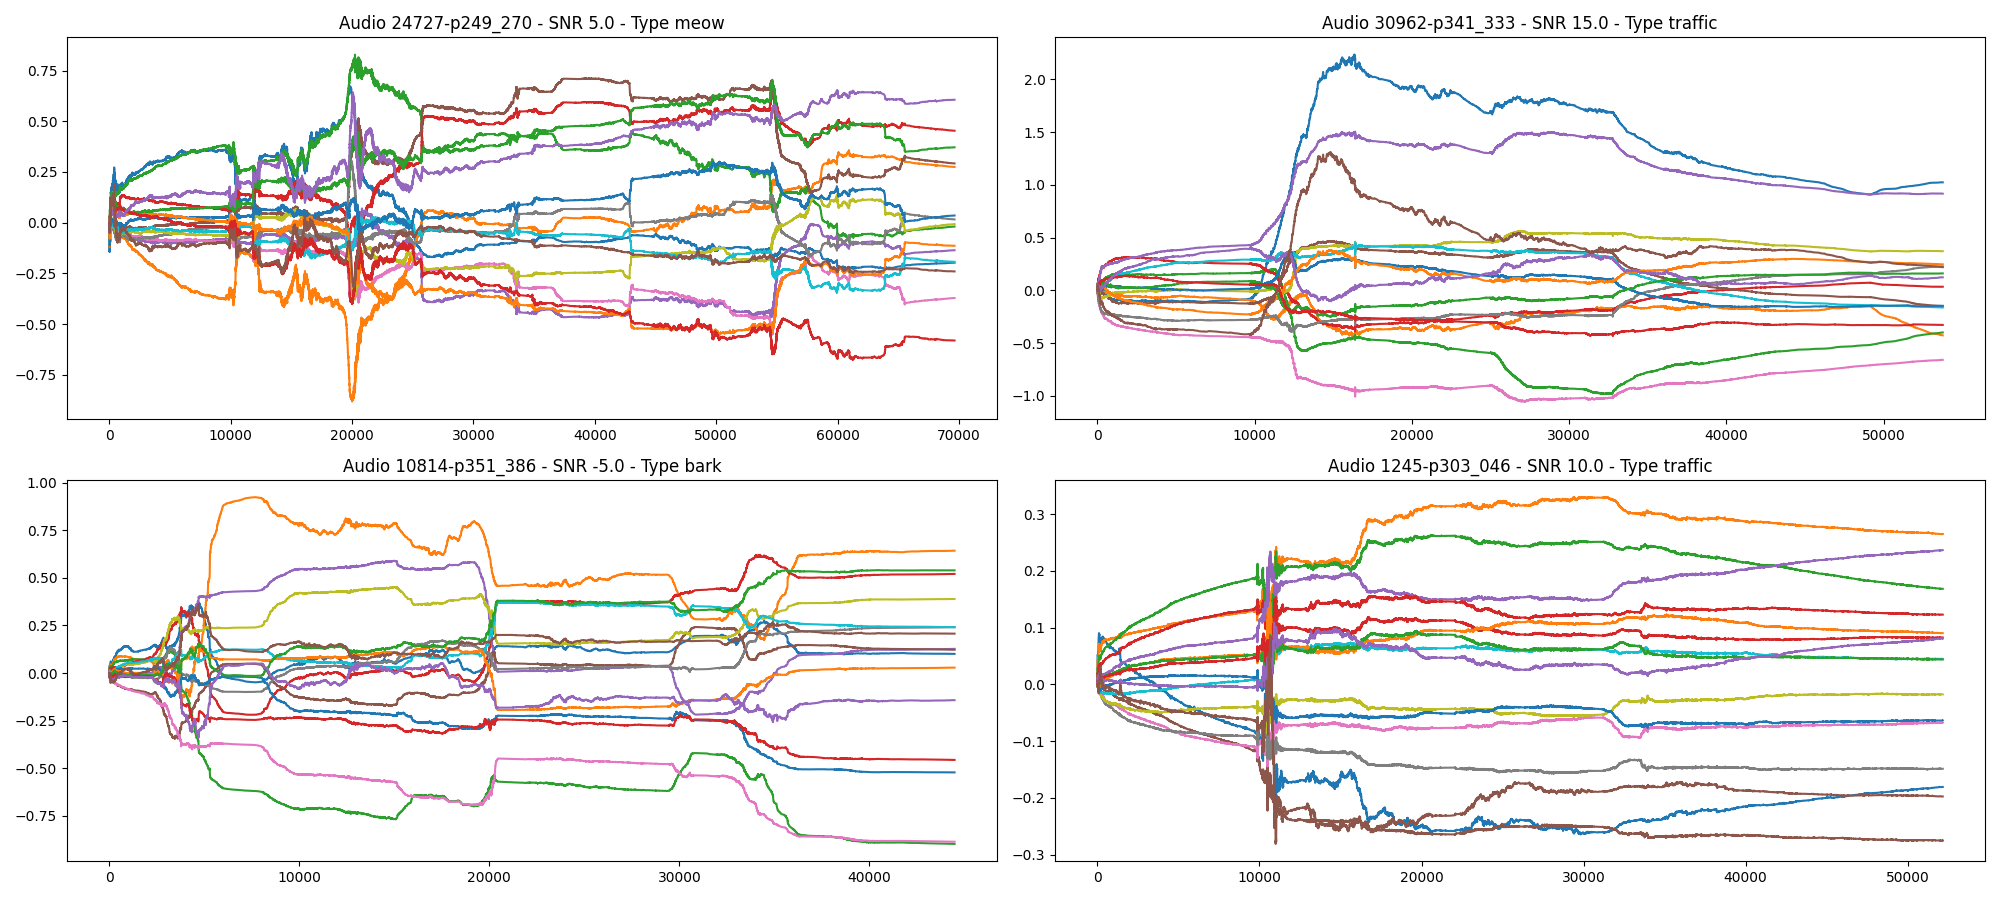
\includegraphics[scale=0.35]{images/ch6/af/weights/weights.png}}
	\caption{Variación de los coeficientes en función del tiempo.}
	\label{fig:ch6_variacion_temporal_de_coeficientes}
\end{figure}

Se observa como los coeficientes se adaptan a medida que cambia la correlación entre los ruidos $n_1(n)$ y $n_2(n)$. Una vez que encuentran la nueva adaptación que minimiza el error, permanecen en un estado estacionario hasta que ocurre un nuevo cambio en el entorno.

\subsubsection{Variación de las señales involucradas en el filtrado}

Al igual que para el caso de los coeficientes del filtro adaptativo, es interesante ver un ejemplo concreto de señal filtrada. La figura \ref{fig:ch6_señal_ruido_habla} muestra un ejemplo de señal de audio filtrada, donde se pueden observar; los coeficientes del filtro, el ruido que corrompió la señal de audio original, el ruido estimado, la señal de habla y la señal de habla estimada . En la figura \ref{fig:ch6_señal_ruido_habla_aumentada} se muestra lo mismo que en \ref{fig:ch6_señal_ruido_habla} pero aumentada entre las muestras $19000$ y $26000$.

\begin{figure}
	\centering
	\centerline{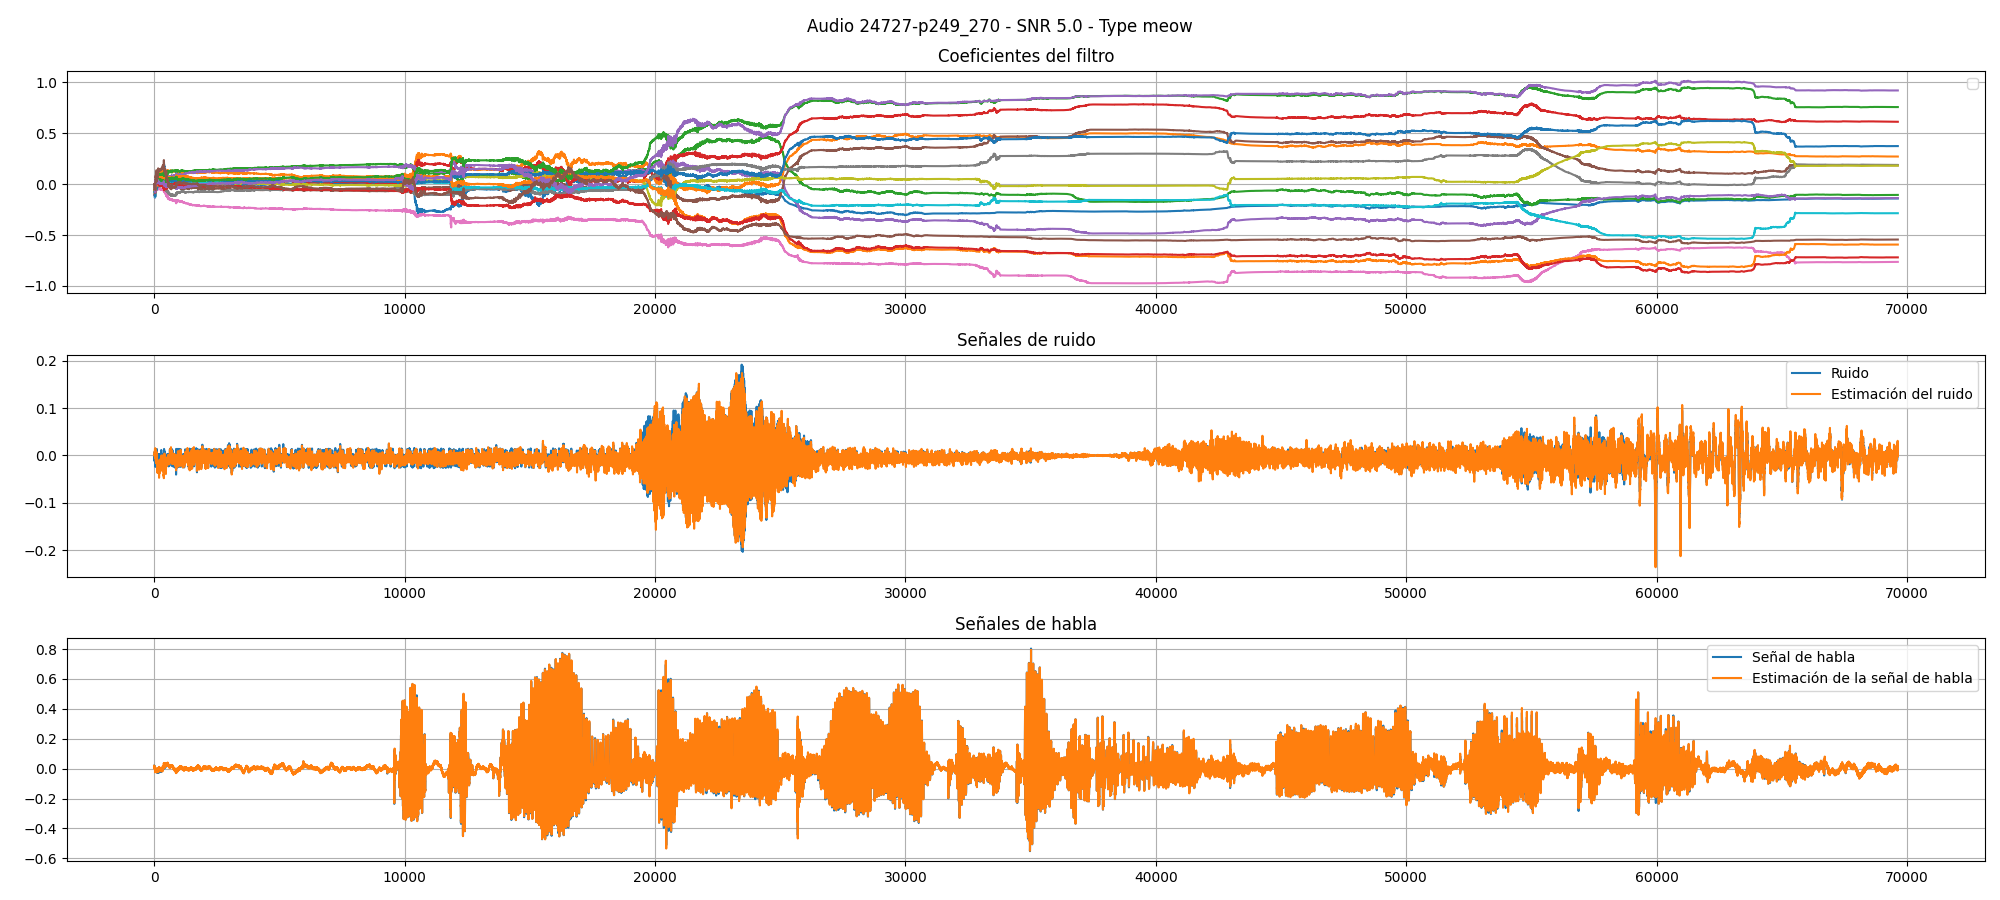
\includegraphics[scale=0.35]{images/ch6/af/signals/signals.png}}
	\caption{Señales de ruido y habla.}
	\label{fig:ch6_señal_ruido_habla}
\end{figure}


\begin{figure}
	\centering
	\centerline{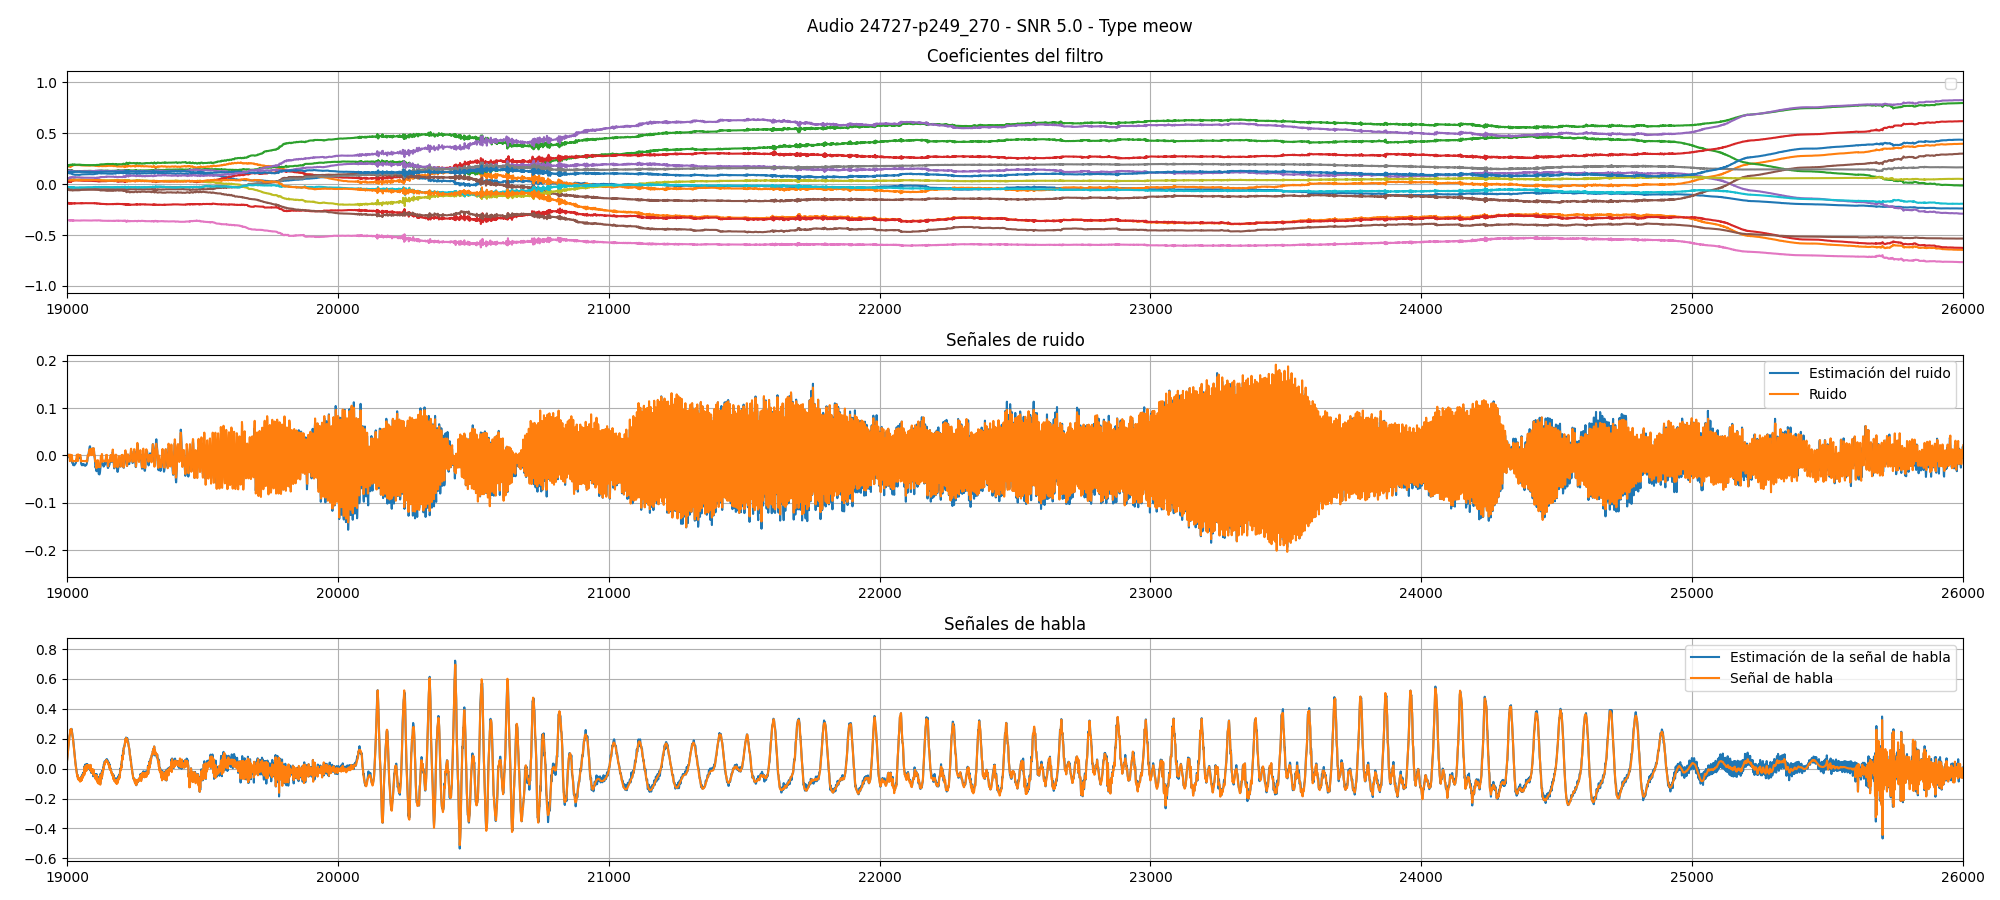
\includegraphics[scale=0.35]{images/ch6/af/signals/zoomed_signals.png}}
	\caption{Señales de ruido y habla aumentadas.}
	\label{fig:ch6_señal_ruido_habla_aumentada}
\end{figure}

En \ref{fig:ch6_señal_ruido_habla_aumentada} podemos ver que tanto el ruido como la señal de habla fueron estimadas con gran precisión.